%%%%
\section{Black Carbon (BC)}

Medidas de BC podem ser realizadas de forma absoluta ou relativa, sendo a
segunda incomparavelmente mais simples e de menor custo que a primeira. 
Um tipo de medida relativa é por refletância, na qual pode-se usar os mesmos 
filtros amostrados para análise elementar por XRF-ED, como PTFE ou 
policarbonato, e é não destrutiva. Todas operações envolvidas nas medições 
consomem algo em torno de um a dois minuto, em média, possibilitando a 
determinação de centenas de amostras em poucos dias.

Outra medida relativa de BC, mais antiga que refletância, é por Aetalômetro,
na qual um feixe colimado de luz monocromática é incidido sobre o
filtro com amostra coletada medindo-se a quantidade luz absorvida via 
atenuação. Medidas relativas de BC são realizadas desde 1980 e ainda hoje são 
intensamente empregadas \citep{targino2016}.

Thermal Optical-Reflectance (TOR) ou Thermal-Optical Transmittance (TOT), 
fornecem medidas absolutas de BC e OC, mas são destrutivas e necessitam de um filtro especial e de um aparato de medidas exclusivo, tendo custo bem mais elevado.

Medidas abosutas, como Thermal Optical-Reflectance (TOR) ou 
Thermal-Optical Transmittance (TOT), necessitam de filtro especial e portanto de 
todo aparato de amostragem exclusivo, são destrutivas e portanto de alto custo.

%%%%
\subsection{Refletância}

Concentrações de BC foram obtidas por refletômetro do tipo 
\textit{Smoke Stain Reflectometer} modelo EEL43D da empresa Diffusion System.
Devido a simplicidade, é tradicionamenbte usado medidas de BC em 
amostras ambientais \citep{lack2014}. 

A técnica baseia-se na propriedade ótica do composto BC possuir alta seção 
de choque 
de absorção de luz na região do visível e é assumido que não existe outras 
partículas que absorvem a luz incidente que não as de BC.

A refletância é uma técnica de medida de BC relativa, pois não mede diretamente
o BC. 

\begin{figure}[H]
  \centering
  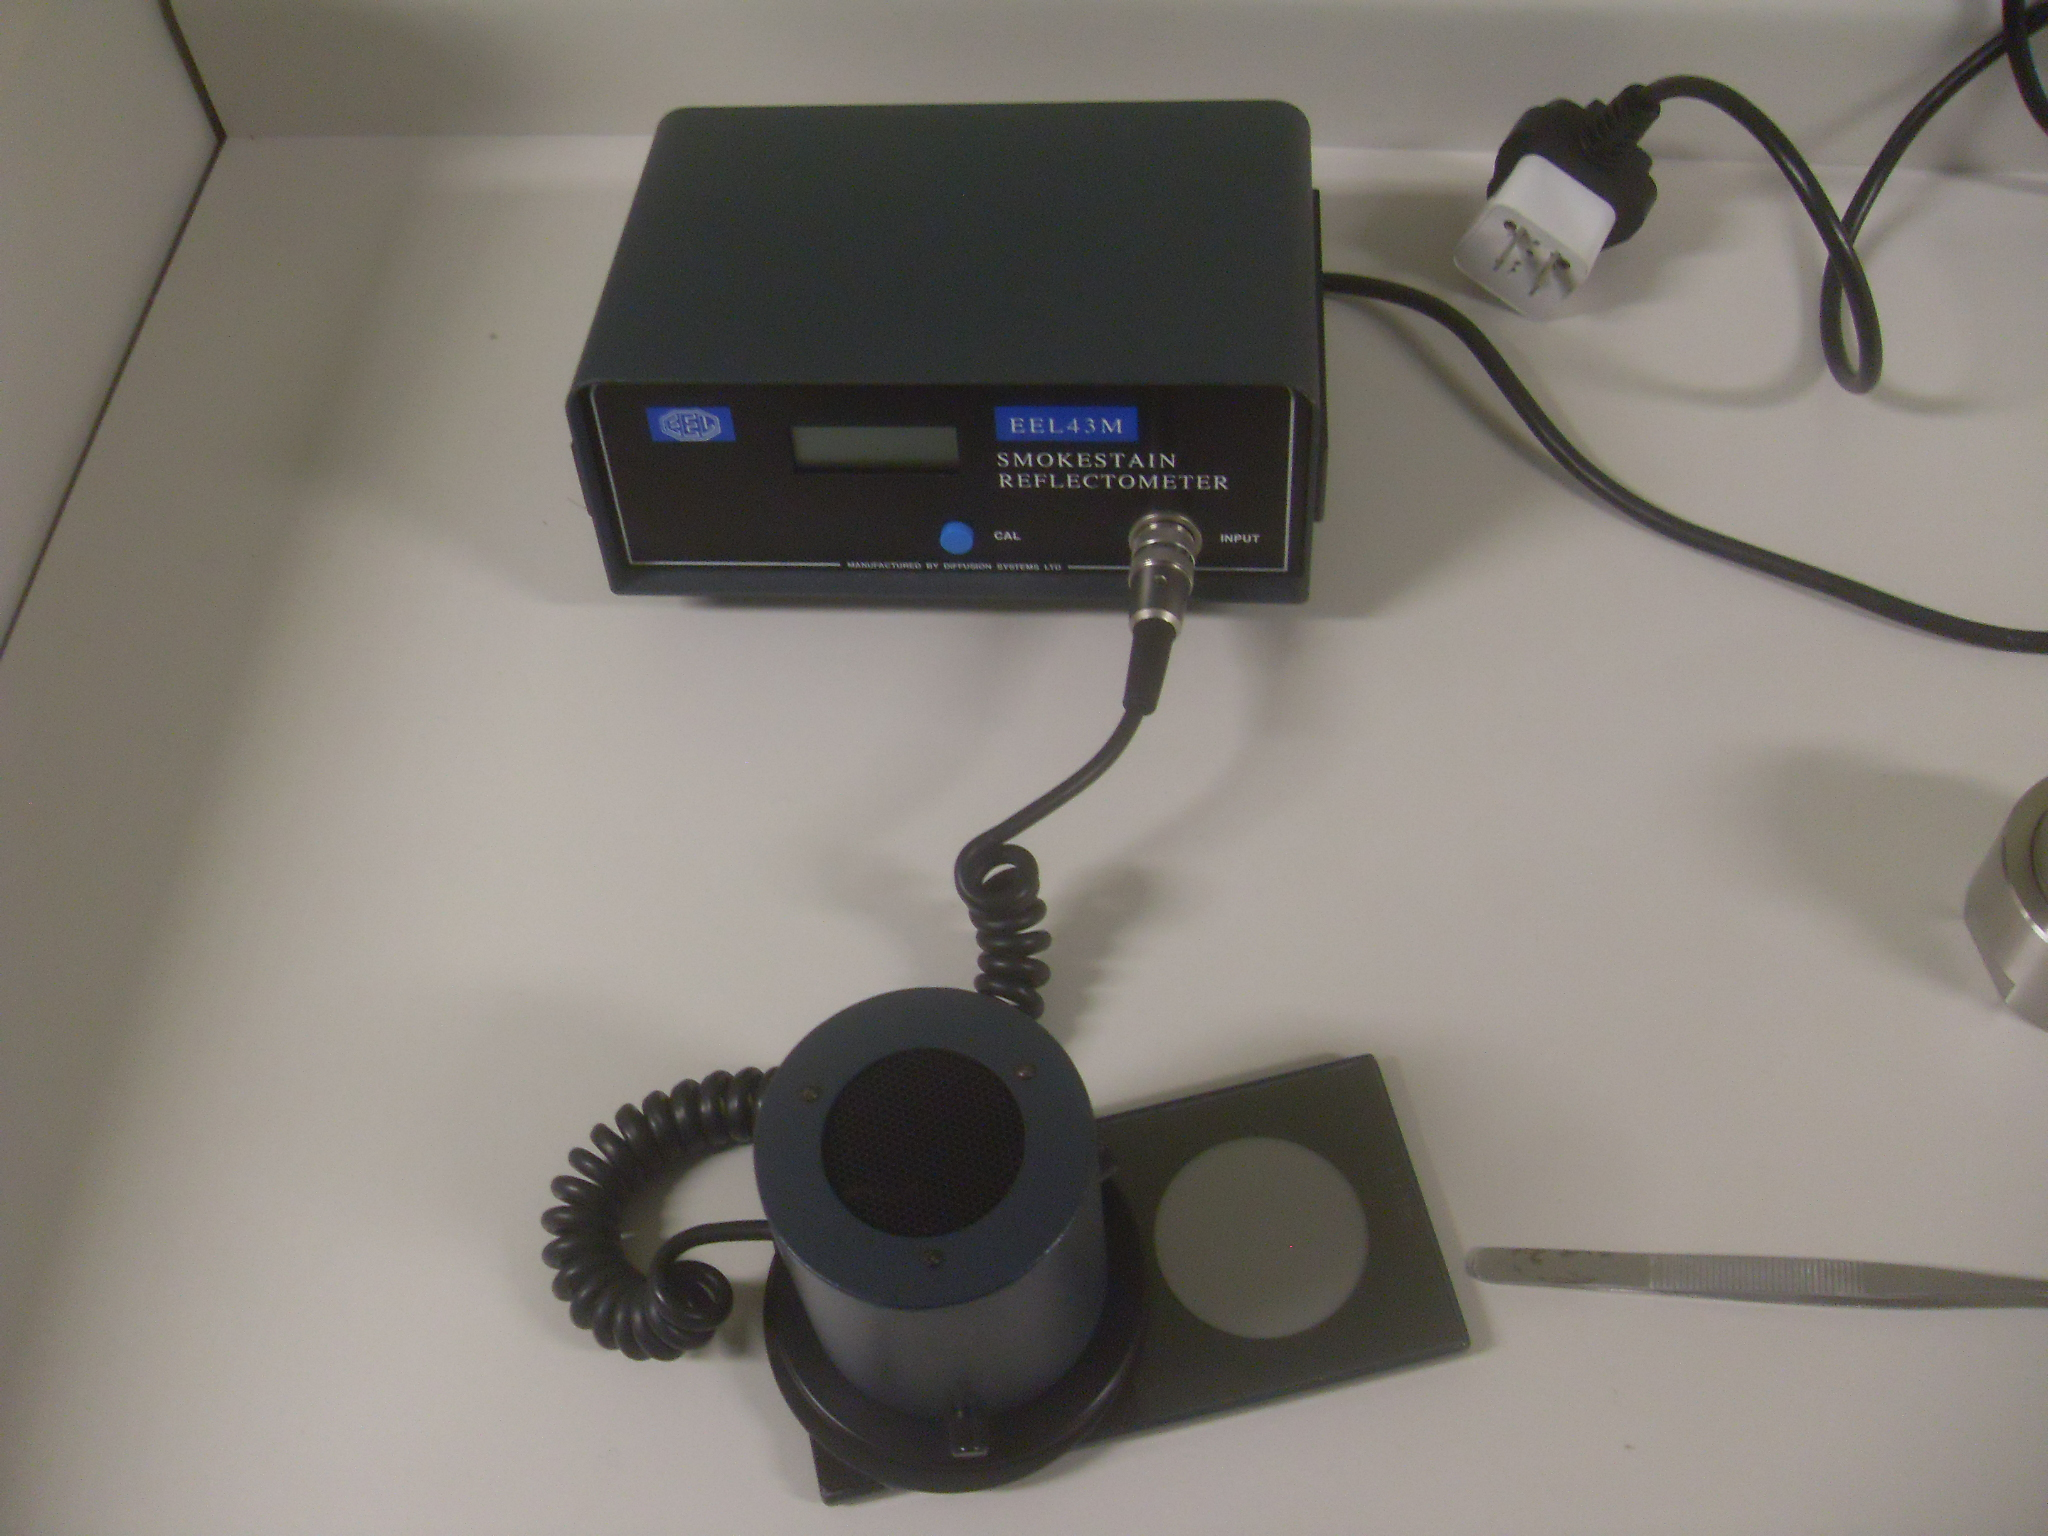
\includegraphics[width=0.5\textwidth]{../inputs/images/refletometro.jpg}
  \caption{Refletômetro Diffusion System modelo ELL43D 
           e peças auxiliares de fixação LAPAt}
\end{figure}

Na refletância, um ponto definido na amostra é ilumindado por lâmpada de 
tungsténio. Parte da luz difusora incidente é absorvida pelas partículas
do filtro e parte refletida. Uma fotocélula com orifício cicurlar, localizada
entre a lâmpada e a amostra, mede a porcentagem da luz refletida (R).
Um filtro branco é usado para fixar o 100\% das leituras a cada 3 medidas.

A luz incidente I decai $-dI/dx$ em qualquer parte camada de partículas na 
amostra:

\begin{equation}
  \label{eq:dIdx}
  -\frac{\delta I}{dx} = I
\end{equation}

Sendo x a espessura da camada de partículas coletas no filtro (e dx uma porção
de x considerada). 
Inserindo-se um coeficiente de proporcionalidade $\alpha$ na equação \ref{dIdx}
e integrando os dois lados da equação, tem-se:

\begin{equation}
  \int_{I_0}^{I} \frac{dI}{I} = - \int_{0}^{x} \alpha dx
\end{equation}

Resultando em uma relação exponencial entre a transmissão do feixe de luz 
que atravessa o filtro e o coeficiente de absorção das partículas:

\begin{equation}
  \label{eq:iso9835}
  I = \frac{I_0}{exp(\alpha x)}
\end{equation}

A equação \ref{eq:iso9835} é regulamentada pela ISO 9835, sendo, I a intensidade 
da luz transmitida, $I_0$ a intensidade da luz incidente, $\alpha$ o coeficiente
de absorção das partículas da amostra e $x$ a espessura da camada de material
depositada no filtro. 

Considerando que a refletância é um caso especial da equação \ref{eq:iso9835} 
em que a luz incidente (ou transmitida) atravessa a camada do material na 
amostra e é refletida na superfície do filtro, passando pela camada de 
partículas da superfície duas vezes, o que siginifica que se pode
multiplicar  por 2, obtendo-se a equação 
\ref{eq:iso9835repletancia}, já com o coeficiente de absorção $\sigma$
isolado.

\begin{equation}
  \label{eq:iso9835refletancia}
  \sigma = \frac{1}{2l} ln\frac{R}{R_0}
\end{equation}
 
%As propriedades ópticas dos filtros de teflon variam sensivelmente. 

%%%%
\subsection{Thermal Optical Transmittance (TOT)}

O Thermal/Optical Transmittance (TOT) é um método absoluto
que mede carbono orgânico (OC) e carbono elementar (EC).
É baseado no princípio  de que diferentes tipos de partículas
compostas de carbono são convertidas para gás em diferentes temperaturas e
condições de oxidação \citep{birch1998}.

Ao aumentar a temperatura, os compostos orgânicos do filtro são volatilizados 
em atmosfera de $He$ não oxidada.
A evaporação do carbono elementar ocorre em temperaturas maiores que 
$580 \degree C$ em atmosfera de $He$ oxidada.
O sistema térmico consiste de um tubo de quartzo dentro de uma bobina aquecida, 
onde a temperatura é controlada por intervalos de tempo.  

Segue-se a sequência de volatilização conforme aumento de temperatura e 
oxidação da atmosfera:

\begin{itemize}
  \item OC1: atmosfera de Hélio na temperatura ambiente $(\pm 25 \degree C)$ até $140 \degree C$
  \item OC2: atmosfera de Hélio em temperatura de $140 \degree C$ até $280 \degree C$
  \item OC3: atmosfera de Hélio em temperatura de $280 \degree C$ até $480 \degree C$
  \item OC4: atmosfera de Hélio em temperatura de $480 \degree C$ até $580 \degree C$
  \item EC1: atmosfera oxidada com temperatura de $580 \degree C$
  \item EC2: atmosfera oxidada com temperatura de $580 \degree C$ até $740 \degree C$
  \item EC3: atmosfera oxidada com temperatura de $740 \degree C$ até $840 \degree C$
\end{itemize}

O gás formado com aumento da temperatura passa por uma placa de dióxido de magnésio 
aquecida e é oxidado para dióxido de carbono, passando por um catalizador de níquel, 
que reduz o dióxido de carbono em metano $CH_4$.
O $CH_4$ é quantificado com uma detector do tipo 
Flame Ionization Detector.

Durante a fase de volatilização do carbono orgânico, parte do carbono elementar
é decomposto pelo processo de pirólise. 
O sistema ótico composto por laser de $He-Ne$ com feixe de intensidade controlada, 
transmissor de fibra ótica e uma fotocélula, contabiliza o carbono elementar
decomposto nesta fase por transmitância.

O carbono elementar total é resultado da soma EC1 + EC2 + EC3 + ECP,
onde ECP é o carbono elementar formado por pirólise. 

Para análises TOT é necessário fazer a coleta em filtros
de quartzo, aumentando os custos e dificultando a logística das medidas, 
pois é necessário montar ponto de medida paralelos.  

Neste trabalho, coletou-se material particulado em filtros de 
quartzo para $\pm 10\%$ dos dias de amostragem e utilizou-se
dos resultados da medida de carbono elementar por TOT 
para inter-calibrar os resultado das medidas de refletância. 
